\section{Progettazione}
Lo sviluppo del progetto si è basato sul pattern \textbf{Model-View} di \textit{Qt} e metodologia mista \textit{top-down} e \textit{bottom-up}. \\
Oltre alla gerarchia, è stato realizzato un Container templatizzato per il contenimento degli oggetti appartenenti alla gerarchia.
Sono stati realizzati inoltre:
\begin{itemize}
  \item Una GUI (Graphical User Interface), basata su classi preesistenti di Qt;
  \item Un Model, il quale si occupa della gestione dei dati del programma, basato anch'esso su classi preesistenti di Qt;
  \item Un filter proxy, che funge da intermediario tra model e view e permette di filtrare i dati per la visualizzazione corretta su ogni tab;
  \item Una classe di Input/Output su file XML.
\end{itemize}

\begin{figure}[H]
  \centering
  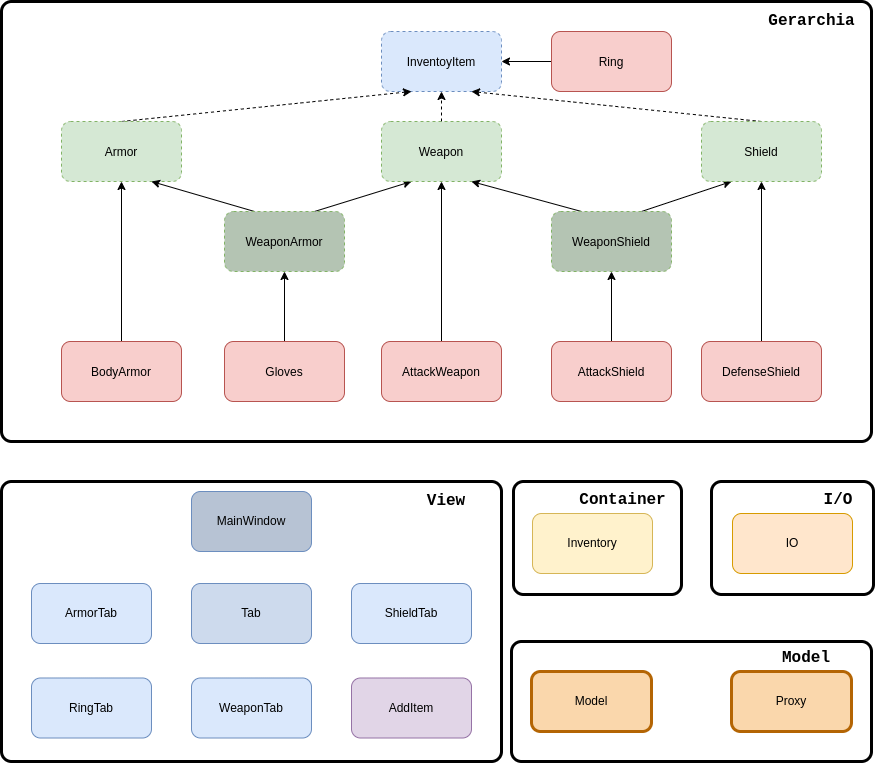
\includegraphics[width = \linewidth]{img/diagramma}
  \caption{Diagramma delle classi di CrownSouls.}
\end{figure}

\subsection{Gerarchia}
La gerarchia è composta dalla classe base astratta \textit{InventoryItem}, dalla quale deriva \textbf{direttamente} la classe concreta \textit{Ring} e \textbf{virtualmente} le classi astratte \textit{Armor}, \textit{Weapon} e \textit{Shield}. Da queste tre classi derivano \textbf{singolarmente} e \textbf{direttamente} le tre rispettive classi concrete \textit{BodyArmor}, \textit{AttackWeapon} e \textit{DefenseShield}. Viene inoltre utilizzata l'\textit{ereditarietà multipla} per la definizione di classi che rappresentano oggetti appartenenti a più tipi; nello specifico, la classe \textit{WeaponArmor} deriva direttamente da \textit{Armor} e \textit{Weapon}, e la classe \textit{WeaponShield} deriva direttamente da \textit{Weapon} e \textit{Shield}. Questa forma di ereditarietà multipla è di tipo \textbf{is-a}, poiché un oggetto WeaponArmor è sia un oggetto Weapon che un oggetto Armor (e lo stesso vale per WeaponShield). Da queste due classi astratte derivano poi rispettivamente le classi concrete \textit{Gloves} e \textit{AttackShield}. \\
Ciascuna classe implementa dei metodi virtuali che riguardano l'impostazione e il recupero delle diverse proprietà degli elementi, e dei metodi virtuali specifici di ogni sottoclasse astratta per il calcolo e l'ottenimento di statistiche basate sulle proprietà. L'utilizzo del polimorfismo in tale contesto viene illustrato in seguito.

\subsection{Container}
Container

\subsection{Modello}
Modello

\subsection{GUI}
GUI

\subsection{I/O}
Input/Output

\subsection{Polimorfismo}
Polimorfismo

\subsection{Scelte progettuali discutibili}
Scelte progettuali
